\documentclass[../main.tex]{subfiles}
\usepackage[utf8]{inputenc}
\usepackage[T1]{fontenc}
\usepackage{graphicx}
\usepackage{longtable}
\usepackage{wrapfig}
\usepackage{rotating}
\usepackage[normalem]{ulem}
\usepackage{amsmath}
\usepackage{amssymb}
\usepackage{capt-of}
\usepackage{hyperref}
\usepackage{float}
\graphicspath{{../}}
\author{Cezary Wieczorkowski}
\date{\today}
\title{Implementacja}
\hypersetup{
 pdfauthor={Cezary Wieczorkowski},
 pdftitle={Implementacja},
 pdfkeywords={},
 pdfsubject={},
 pdflang={Polish}}
\begin{document}


\section{Implementacja stanowiska}

\subsection{Część sprzętowa}

\subsubsection{Enkoder oraz wyświetlacz}

Sposób podłączenia wyświetlacza LCD oraz enkodera został przedstawiony na rysunku \ref{fig:lcd_enc_connection}.

\begin{figure}[H]
    \centering
    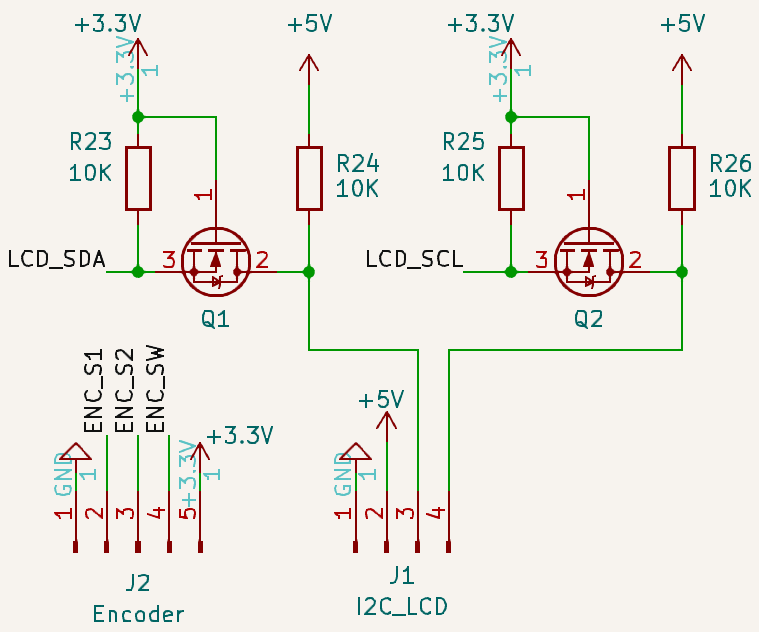
\includegraphics[width=\linewidth]{lcd_schemat.png}
    \caption{Schemat połączeń enkodera oraz wyświetlacza}
    \label{fig:lcd_enc_connection}
\end{figure}

Obsługa modułu enkodera wymaga podłączenia zasilania, sygnałów A i B - wyjść impulsów enkodera oraz sygnału SW - wyjścia przycisku. 
Sygnały A, B oraz SW zostały podłączone bezpośrednio do końcówek GPIO mikrokontrolera. Obsługa wyświetlacza wymaga podłączenia 
zasilania oraz sygnałów SCL i SDA dla interfejsu I2C używanego do komunikacji z ekspanderem I/O PCF8574 obsługującym wyświetlacz. 
Pierwotnie wyświetlacz oraz ekspander zasilono tak z napięcia 3,3 V. Podczas wstępnego uruchomienia zestawu zauważono, że
obraz na wyświetlaczu jest niewyraźny. Było to spowodowane zbyt niskim napięciem zasilania dla poprawnego funkcjonowania podświetlenia
wyświetlacza. Po zwiększeniu napięcia zasilania do 5 V problem ustąpił. Zmiana wartości napięcia zasilania wymagała zastosowania
konwerterów poziomów logicznych na liniach SCL i SDA, ponieważ mikrokontroler RP2040 pracuje z napięciem 3,3 V. Zastosowany konwerter 
poziomów logicznych jest oparty o tranzystor MOSFET typu N. Ważną właściwością tego typu konwertera jest możliwość konwersja poziomów w obu \
kierunkach która jest w tym wypadku konieczna gdyż linia SDA jest linią dwukierunkową.

\subsubsection{Diody LED oraz przyciski}
Diody LED są sterowane przez trzy rejestry przesuwne 74HC595. Zgodnie z notą aplikacyjną \cite{ti:74hc595}
w celu sterowania układem należy wykonać następujące połączenia:

\begin{itemize}
    \item VCC - zasilanie 3,3 V
    \item GND - masa
    \item SER - linia danych, w pierwszym układzie podłączona do końcówki GPIO mikrokontrolera natomiast w kolejnych 
    układach podłączona do wyjścia danych  poprzedniego układu
    \item $\overline{SRCLR}$ - linia resetu podłączona na stałe do napięcia zasilania
    \item SRCLK - linia zegara podłączone do końcówki GPIO mikrokontrolera
    \item RCLK - linia zegara rejestrów wyjściowych podłączone do końcówki GPIO mikrokontrolera
    \item $\overline{OE}$ - włączenie wyjścia podłączone na stałe do masy
\end{itemize}

Na wyjściu układu w stanie wysokim pojawi się napięcie 3,3 volta, zastosowane diody LED charakteryzuje napięcie przewodzenia około 2 V. Charakterystyka
zależności prądu od napięcia diody rośnie bardzo szybko po przekroczeniu napięcia przewodzenia. W celu ograniczenia prądu przepływającego przez diodę
stosujemy szeregowy rezystor. Wartość tego rezystora obliczamy z następującego wzoru: 
\begin{equation}
    R = \frac{V_{CC} - V_{LED}}{I_{LED}} = \frac{3,3 V - 2 V}{10 mA} = 100 \Omega
\end{equation}

\begin{figure}[H]
    \centering
    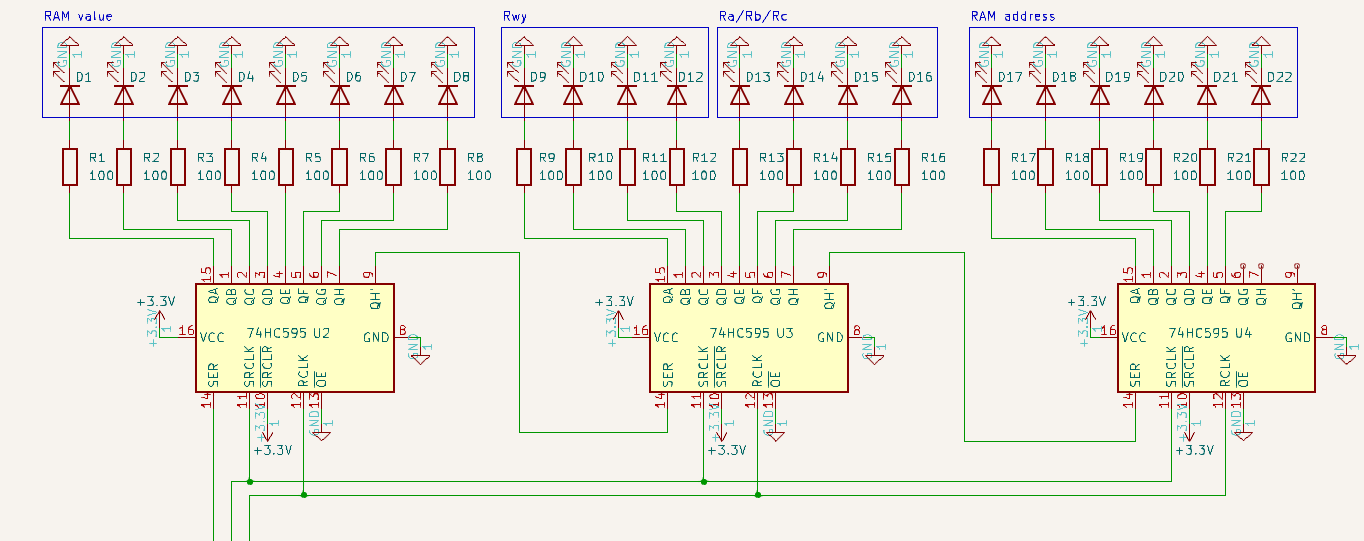
\includegraphics[width=\linewidth]{led_schemat.png}
    \caption{Schemat połączeń rejestrów wraz z diodami LED}
    \label{fig:led_connection}
\end{figure}

Przełączniki zostały podłączone bezpośrednio do końcówek GPIO mikrokontrolera. Włączenie przycisku powoduje zwarcie linii GPIO z masą
co zostanie odczytane jako stan niski na danej końcówce. Stan wysoki w przypadku rozwarcia przycisku jest  wymuszany przez wbudowane
w port wejściowy mikrokontrolera rezystory podciągające do napięcia zasilania.

\begin{figure}[H]
    \centering
    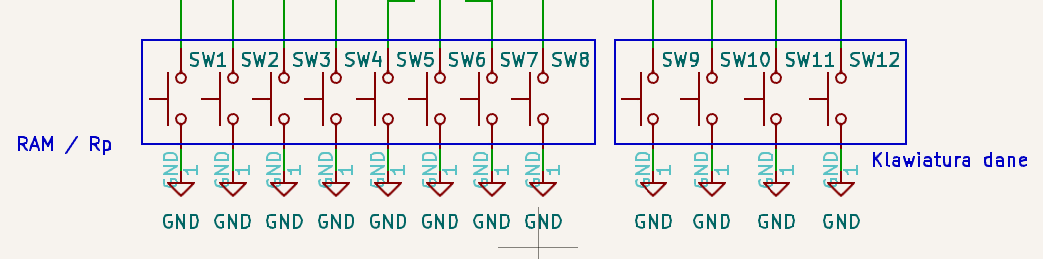
\includegraphics[width=\linewidth]{button_schemat.png}
    \caption{Schemat połączeń przycisków}
    \label{fig:button_connection}
\end{figure}

\subsection{Konstrukcja prototypu}



\begin{figure}[H]
    \centering
    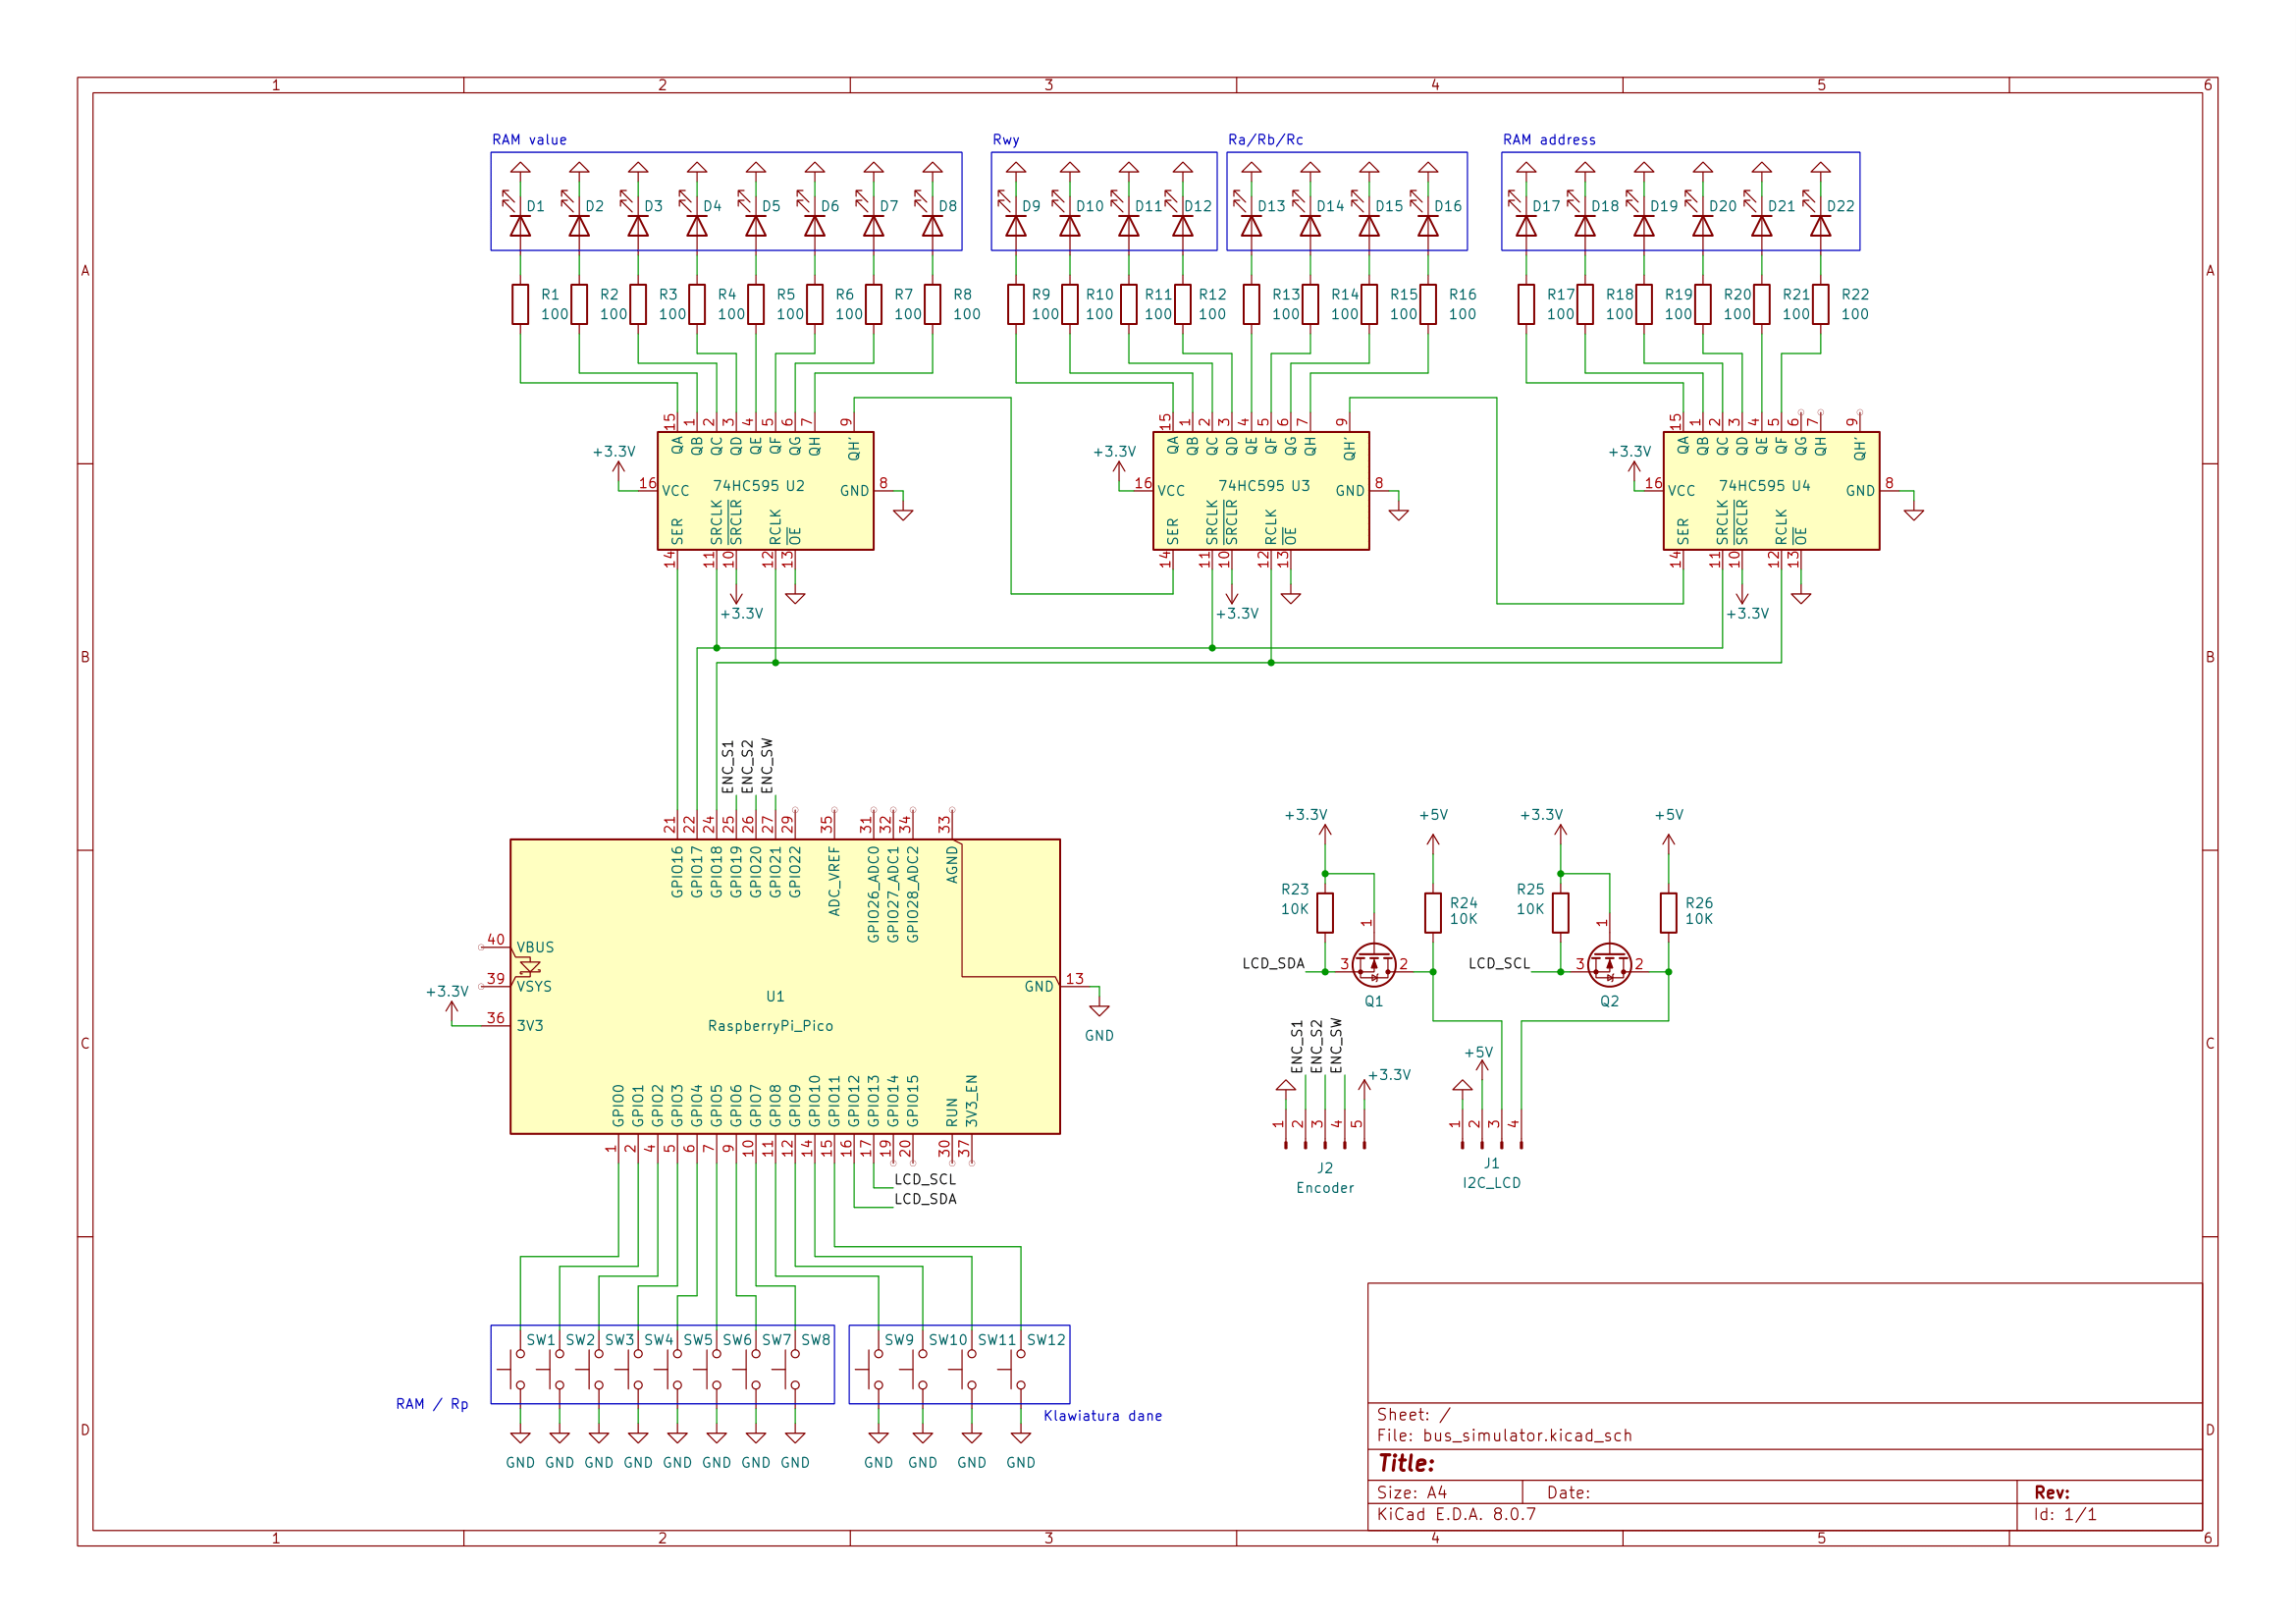
\includegraphics[width=\linewidth]{schemat.png}
    \caption{Schemat elektryczny zestawu}
    \label{fig:electrical_schematic}
\end{figure}


\subsection{Część programowa}

\subsubsection{Obsługa rejestrów oraz przycisków}



\subsubsection{Symulacja elementów zestawu}



\end{document}